The first step to answer the research question was to choose an application to develop. This chapter presents the criteria used in the selection process and the application chosen: home automation.

\section{Selection Criteria}\label{sec:selec_cri}

The application developed during the research should ideally display characteristics inherent to \acs{iot} applications~\cite{survey,survey2,survey3}. Although, some of there characteristics --- energy consumption, performance and security --- were not considered during the research. These aspects were ignored because the development of \gls{iTasks} overlooked them. Additionally, some criteria were added based on the research question.

The following criteria were used to choose an application:

\paragraph{Suitable} The application should solve a problem that is suitable for \gls{mTask}. This narrows the choice to \ac{iot} applications that can be developed for platforms supported by \gls{mTask}.

\paragraph{Non-trivial} Trivial applications (e.g. an \acs{led} blinking) were previously developed~\cite{martthesis}. Therefore, the application should not solve a trivial problem --- e.g. a simple hallway  motion-activated light sensor. It should go beyond a purely reactive system. It does not have to solve a novel problem, but its development should be adequately challenging.

\paragraph{Simple} Due to time constraints, it should be simple enough to be developed during this research. Since building a full-pledged application is not the goal of the research, some concerns as feature completeness, user experience design and security are not taken into account. Its source code should not be too complex.

\paragraph{Interesting} It is not enough that the application is suitable and technically good. It should tackle an existing, interesting problem. Ideally, a problem which users inserted into the application domain would be willing to pay for a solution.

\paragraph{Significant} The application should somehow improve the environment it is inserted into. Examples are accelerating an assembly line, saving commute  time, improving one's health or well being or reducing operational cost.

\paragraph{Comprehensible} Its domain and main features should be easily understandable by non-domain experts. Its functionality details and operational features might require specific knowledge, but the application should be easily described on a high level to someone who is not inserted in its domain. Comprehensibility is relevant because it improves the application and therefore the research's reachability. 

\paragraph{Robust} The application should be able to handle errors to some extent. It should at least be able to detect and communicate device disconnection. Ideally, it would automatically migrate tasks from disconnected devices to available devices whenever possible. 

\paragraph{Highly connected} It should support multiple devices simultaneously. These devices should be able to exchange information (e.g. sensor values) when suitable. Ideally, the devices would be connected wirelessly.

\paragraph{Dynamic} The application should not be static. Given that the interpreted version of \gls{mTask} (Section \ref{sec:int_mtask}) is being explored, its dynamic nature should be exploited. The application domain should naturally allow dynamicity. Ideally, tasks would be sent to and removed from devices regularly.

\paragraph{Diverse} It should use as many peripherals as possible. Since \gls{mTask} targets microcontrollers, it is important that a diverse group of sensors and actuators is used. The application should not restrict itself to a couple of peripherals. 

\paragraph{Extensive} The application should use \gls{mTask} features extensively. Given that it is testing \gls{mTask}'s capabilities, it is important that the application tests as many \gls{mTask} features as possible. There is a correlation between the number of features used by the application and the certainty about \gls{mTask}'s abilities.

\section{Home Automation}

Many potential \ac{iot} applications were considered to be developed during research. After a systematic selection process based on the selection criteria described on Section \ref{sec:selec_cri}, a home automation solution was chosen. A detailed analysis of why this domain was chosen is presented in Section \ref{sec:app_analysis}.

Home automation might refer to different levels of automation of home tasks. By definition, any tool or machine that automates a home task constitutes a home automation solution. Historically, home automation became popular with the advent of distributed electricity. Daily tasks as dishwashing and drying clothes were automated by appliances that today are common in many households around the world.

In the last decades, home automation gained another meaning with the invention of electronic solutions that control virtually any electronic in a house. Lighting, air conditioners, heaters, entertainment systems and doors are common components controlled by home automation solutions. Frequently, these systems are composed by a central control unit with a user interface (e.g. computer, tablet, smartphone, wall control panel), a communication channel (e.g. Bluetooth, \acs{lan}, Internet, infrared) and devices to be controlled (e.g. lamp, air conditioning unit, doors, TV, appliances).

Automated tasks might be as simple as turning a light on when someone enters the room, controlling the heater based on a target room temperature, locking the main door at a set time and closing the curtains based on the amount of natural light outside. They might also be more elaborated as automatically turning the coffee maker on at 8:00 AM on work days, but only if somebody is at home.

\section{Application Description}\label{sec:app_desc}

The home automation application developed is called Autohouse. It enables and manages the automation of a home (hereafter referred to as \textit{smarthome}) using \gls{mTask}. A smarthome is composed by rooms that can be added and removed by its user. Each room contain devices (called \textit{units} in the application) that execute tasks chosen by the user. 

A smarthome is managed via the control panel, a web interface that can be accessed using a web browser. Multiple instances of the control panel can run simultaneously. There, the user has access to the main features of the application:

\begin{itemize}
    \item Manage home: add and remove rooms to the smarthome.
    \item Manage room: add and remove units to a room.
    \item Send task: send a new task to one of the available units.
    \item Inspect unit: see which tasks are running on a unit.
\end{itemize}

\subsection{Architecture}

Autohouse is a centralized solution: a server (ideally located in the home) is the central communication hub for both users and devices. User communication is accomplished via the web control panel, which is hosted in the server. Device communication is accomplished via the \gls{mTask} library and its communication protocol described in Section \ref{sec:mtask_com_prot}. Figure \ref{fig:autohouse_arch} displays an example architecture of Autohouse deployed on a home with three units. 

\begin{figure}[H]
\begin{center}
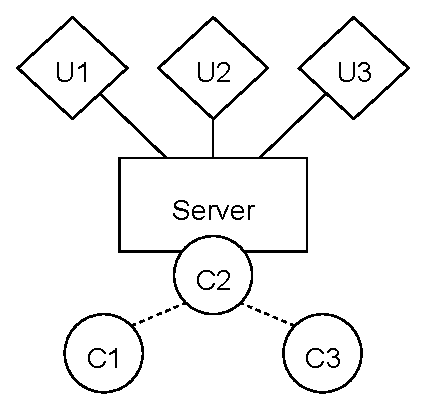
\includegraphics[scale=1.0]{thesis/img/autohouse_arch.eps}
\end{center}
\caption{Autohouse Architecture}
\label{fig:autohouse_arch}
\end{figure}

In Figure \ref{fig:autohouse_arch}, units are represented as diamonds, the server is represented as a rectangle and clients accessing the web control panel are represented as circles. Rooms are just an abstraction layer to ease the use of Autohouse and therefore are not represented in its architecture. Units are microcontrollers equipped with peripherals (sensors, actuators) and with a communication interface. The server can be any computer with networking capabilities that is supported by \gls{clean} and that has enough resources to run the application. A client is a device accessing the control panel using a web browser. Note that the server itself may be a client, since it can access the control panel via a web browser. In addition, if the server is exposed to the Internet, the control panel can be accessed remotely. 

Communication between the server and the units must be persistent (represented by the continuous line between them in Figure \ref{fig:autohouse_arch}). If the communication is interrupted, the server interprets it as a disconnection. Communication between the server and the clients can be transient (represented by the dotted line between them in Figure \ref{fig:autohouse_arch}). Since clients are just managing the application, their connection does not have to be persistent. 

Following one of the criterion introduced in Section \ref{sec:selec_cri}, units should connect to the servers wirelessly. The \gls{mTask} library supports two types of connections: Serial and \acs{tcp}. Although, which technology is used to establish these connections is irrelevant to the end user. Therefore, Autohouse is technology agnostic in regard to communication between units and the server. Units can, for example, establish a serial connection via Bluetooth or a \acs{tcp} connection via WiFi. As a consequence, Autohouse does not enforce a wireless connection between the units and the server. The user decides which communication technology is more adequate to their needs.

\subsection{Tasks}

The main purpose of Autohouse is to send automation tasks to units so they can be executed without human supervision. Therefore, the tasks the application supports play a key role in Autohouse. The application has a list of predefined tasks that are relevant to the house automation domain. The user can pick tasks from this default task list and select a unit to send it to. The standard task list might be extended by adding new tasks to the \texttt{Programs} module. The \gls{autohouse} standard tasks are listed below.

\begin{itemize}
    \item Control a light based on a switch. 
    \item Turn a light on when movement is detected.
    \item Lock a door when it gets dark.
    \item Open the garage door if a car is reversing.
    \item Turn a fan on when it gets humid enough, but turn it off when something is about to hit it.
    \item Open and close windows based on a target temperature range.
    \item Open and close curtains based on the amount of light in the room.
    \item Manage the air conditioning unit and the heater based on a target room temperature and on the actual room temperature.
\end{itemize}

\subsection{Devices}\label{sec:autohouse_devices}

Three platforms are supported by mTaks: \gls{arduino}, \acs{posix} and \gls{mbed}. \gls{arduino}~\cite{arduino} was chosen as the main platform for Autohouse. \gls{arduino} is an open-source electronics prototyping platform which has single-board microcontrollers specifications and software to support them. It was chosen because of its open-source nature, popularity, well-established community and open-source code availability.

The \gls{arduino} platform currently has many boards with different specifications and purposes. The \gls{arduino} Uno Rev3\footnote{Arduino Uno Rev3. Available at \url{https://store.arduino.cc/arduino-uno-rev3}. Accessed on August 26th 2018.} was chosen as the target device because of its popularity, extensibility (using shields\footnote{Arduino Shields. Available at \url{https://www.arduino.cc/en/Main/arduinoShields}. Accessed on August 26th 2018.}), cost and limited resources. The \gls{arduino} Uno is based on the ATmega328P microprocessor, which has only 2 KB of RAM. This memory limitation is a desired characteristic, given that \gls{mTask}'s suitability for microcontrollers is being tested and that such devices might have extremely limited resources. The \gls{arduino} Uno operates at a frequency of 16 MHz, has 6 analog pins, 14 digital pins, 32 KB of flash memory and a built-in \acs{led}. Its digital and analog pins are often used to interface with peripherals, including sensors and actuators. 



Sensors and actuators are extremely relevant to Autohouse because they allow the application to interface with the real world without human interference. Examples of sensors are temperature, humidity and movement sensors. Examples of actuators are buttons, switches, \acsp{led} and motors.

\subsection{Sensors}

\gls{autohouse} relies on the interpreted \gls{mTask} and its \gls{arduino} client for peripheral support. Therefore, it supports the same sensors the \gls{arduino} client does. Digital and analog pins can be controlled explicitly, but \gls{mTask} also provides native support for some sensors. Namely, for the DHT22 temperature and humidity sensor, the HCSR04 ultrasonic sensor, digital light sensor, Grove analog light sensor (P) V1.1 and \ac{pir}. Native sensor support allows programming in a high level of abstraction, in which sensor values represent their semantics. For example, reading from a temperature sensor returns a \texttt{Temperature}, an \acs{adt} that represents temperature in Celcius. Some of these sensors were not previously supported by \gls{mTask}. Section \ref{sec:new_peri} describes how these peripherals were incorporated into \gls{mTask}.

\subsection{Actuators}

Similarly to sensors, \gls{autohouse} relies on the interpreted \gls{mTask} and its \gls{arduino} client for actuator support. Some actuators (e.g. switches, buttons) can be directly controlled through pins and therefore do not require custom support. Other actuators, though, require custom support to be practically used. The interpreted \gls{mTask} provides native support for \acs{lcd} displays (to print integers only), \acsp{led} and servos. Servos were not previously supported by \gls{mTask}. Section \ref{sec:new_peri} describes how servos were incorporated into \gls{mTask}.

\section{Application Analysis}\label{sec:app_analysis}

The selection process that chose Autohouse as the research application was guided by the selection criteria presented in Section \ref{sec:selec_cri}. In this section, the Autohouse choice is motivated by analyzing the application under those same criteria.

\paragraph{Suitable} Autohouse is suitable for \gls{mTask}. Its components are small devices connected to a server that (if connected to the internet) can be accessed anywhere. In addition, Autohouse targets \gls{arduino} Uno, a board supported by \gls{mTask}.

\paragraph{Non-trivial} It is not a trivial application. The complexity of Autohouse goes beyond a simple reactive system. It is an application with a user interface where its user can dynamically add devices and send automation tasks to such devices. Its tasks can be simple reactive tasks but can also contain complex logic based on input from different sensors and devices.

\paragraph{Simple} Autohouse was simple enough to be developed during the research. Thanks to the prototyping nature of \gls{iTasks}, its development could abstract from many technical details and focus on design decisions.

\paragraph{Interesting} Home automation is becoming increasingly popular and its industry is growing consistently\footnote{Global Home Automation Market Growth Opportunities 2017-2022 - Market is expected to reach an estimated \$75.2 billion. Available at \url{https://markets.businessinsider.com/news/stocks/global-home-automation-market-growth-opportunities-2017-2022-market-is-expected-to-reach-an-estimated-75-2-billion-1007431226}. Accessed on August 27th 2018.}. There is no industry standard and the market is highly fragmented. Therefore, Autohouse solves an existing, interesting problem.

\paragraph{Significant} Autohouse might improve many aspects of its user's life. For example, Autohouse tasks can save time (e.g. automatically opening the garage door when a car moves backwards). They can also save energy (e.g. automatically turn off the lights and electronics when nobody is home). They might also improve the user's well being (e.g. automatically regulate room temperature) and health (e.g. open the windows when the air quality inside is poor). In addition, tasks can be simply convenient (e.g. open the curtains when it is bright outside).

\paragraph{Comprehensible} The home automation domain is comprehensible to most people. We all live in homes and can relate to most of the tasks Autohouse offers. Therefore, no explanation of the application domain is required to comprehend it. 

\paragraph{Robust} Autohouse is a robust application when it comes to device disconnection. If a unit is disconnected from the server, the system migrates the tasks that were running on that unit to another, suitable unit. The application does not support server fault tolerance. Although the distributed version of \gls{iTasks} could have been used, Autohouse runs on the single server version instead~\cite{distributed}.

\paragraph{Highly connected} Autohouse supports multiple simultaneous devices. In the home automation domain, having many devices simultaneously connected is not only common, but encouraged. Wireless connections are supported but as explained in Section \ref{sec:app_desc}, Autohouse does not enforce them. 

\paragraph{Dynamic} The Autohouse system allows for dynamic addition and removal of devices. In addition, a user might send tasks to devices dynamically. Home automation is a domain that naturally requires dynamicity. It is expected that Autohouse users create and delete tasks on a daily basis.

\paragraph{Diverse} Autohouse supports five different sensors and three actuators. Therefore, in total, eight peripherals are integrated into the application. Although this number is small when compared to some commercial applications out there, it is enough to display Autohouse's diversity.

\paragraph{Extensive} The application tests \gls{mTask} features thoroughly. Regarding the \gls{mTask} language, \gls{autohouse}'s default tasks use all of the language constructs implemented by the \gls{mTask}'s interpreted view (Section \ref{sec:int_mtask}). In addition, it makes use of \gls{mTask} functionality to connect to devices and to send tasks to it. Autohouse benefits from \gls{mTask} abstraction layer over devices and does not handle them directly.

